\documentclass[11pt,a4paper,english]{article}
\usepackage[english]{babel}
\usepackage{marginnote}
\usepackage[utf8]{inputenc}
\usepackage[top=1in]{geometry}

\usepackage{graphicx} %behandle grafikk
\usepackage{float}
\usepackage[hidelinks]{hyperref} %trykkbar referering
\usepackage{gensymb}

\usepackage{todonotes} % for drafting

\newenvironment{loggentry}[2]% date, heading
{\noindent\textbf{#2}\marginnote{#1}\\}{\vspace{0.5cm}}


\title{UNIK4690 Project}
\author{
  Akhsarbek Gozoev  - akhsarbg \\
  Sadegh Hoseinpoor - sadeghh\\
  Key Long Wong - keylw
}


\begin{document}

\maketitle
\section{Project description}
\textbf{The purpose of the software is to recognise text from any
surface with uneven lighting. Hence this falls under the ``Optical character recognition'' (OCR) problem}

\noindent \\ As OCRs are still a challenging task even for companiese like
Google, ref. reader to Googles OCR translator application on smartphones;
``Transalte'', drawbacks such as; difficulty finding all the text on the photo
becasue of lighting, noise etc., therefore we will have to limit our software
significantly.

\subsection{Initial limitations}
\begin{itemize}
 \item{English alphabet + numbers [0-9]}
 \item{Homogeneous background}
 \item{Computer printed text}
\end{itemize}

\subsection{Project components}
The group have come to the conclusion that the OCR software has 3 main
components to it.
\begin{enumerate}
 \item{\textit{Text segmentation}}
 \begin{itemize}
  \item{Finding text on an image and returning the text segments}
 \end{itemize}
 \item{\textit{Preprocessing}}
 \begin{itemize}
  \item{Do preprocessing on the segmented text; rotation, symbol segmentation,
  etc.. (preprocessing from its definition, should be done first, however
  because of simplification we assume we manage to segment out text first.)}
 \end{itemize}
 \item{\textit{Classification}}
 \begin{itemize}
  \item{Classification of the symbols}
 \end{itemize}
\end{enumerate}
\noindent \\ Additionally there is one more very important component for this
OCR software to work, \textit{\textbf{labled data}}. Even though one might not
need to code for this part, a good pool of labeled data is needed to be able to
classify symbols. More on this later.
\noindent \\ (4. \textit{Data classification - Gathering labeled data to train a classification algorithm})

\subsection{Component description}
This section we will describe our thoughts on how we plan to solve each
component, in the form of algorithms, APIs, and datasets. Note that this is our
initial thoughts, not necessary the solution we will end up implementing.

\noindent \\ As we want to test proof-of-concept while we are coding, we will
be making several simplifications. These simplifications will be described
further under each component.



\subsubsection{Text segmentation}
\todo[inline]{\textbf{Key fyll ut dette her} \\
. \\
. \\
. \\
. \\
. \\
. \\
}
\subsubsection{Preprocessing}
\noindent \\ \textbf{Description}
\noindent \\

\subsubsection{Classification}
\noindent \\ \textbf{Description}
\noindent \\ At this point because of avalible knowledge and the intrest in
Convolutional Neural network (CNN), we ended up trying to solve this part
both with a CNN, and a Multilayer Peceptron (MLP or Deep neural network (DNN)).

\noindent \\ \textbf{Deep Neural Network}
\noindent \\ Multilayer peceptron neural networks are relatively straight
forward to code, however the challinging part is to decide on good
hyperparameters and to not overfit our network.
\noindent \\ \textbf{hyperparameters}
\noindent \\
\begin{itemize}
 \item{Number of Layers}
 \item{Number of nodes in each layer}
 \item{Activation functions}
 \item{Loss function}
 \item{Optimization function}
 \item{Learning rate}
 \item{Initialization of the weights and biases}
 \item{Number of epochs}
\end{itemize}




\noindent \\ \textbf{Convolutional Neural Network}


\noindent \\ \textbf{Limitation - proof of concept}


\subsubsection{Labled Data}
\noindent \\ \textbf{Description}
\noindent \\
Labled data is needed because our classifiers need to be trained to understand
the difference between the charecters. This is usually done by training a
classifier with a set of training data, labels are needed in our case,
since it is a supervised machine learning algorithm we want to use. As the
training data is used to train the software, we will need data to test our
software as well, hence the need for test data. The test data is used to get a
measure of what the error rate of our software is, based on the results we
can then tune the hyperparameters to get a better/smaller error rate. Lastly
we will need validation data. This is an independent dataset that the software
is not familiar with. The accuracy of the software on the validation set will
then be a measure of how good the software can classify the characters.

\noindent \\ \textbf{Limitation - proof of concept}
\noindent \\
As we have limited us to the English alphabet and numbers ranging from [0-9],
we will need labeled data for each of these 36 characters; training, test and
validation sets. As the concept of classifying only numbers vs all 36
charecters does not differ that much, we will first see if we can solve the OCR
problem with just numbers. Therfore we only need a dataset containing numbers
at first. Thereafter we will search for a dataset containing all the characters
we need.

\noindent \\ \textbf{Dataset}
\noindent \\
\noindent \\ \textbf{MNIST}
\noindent \\ This is a dataset containing handwritten numbers [0-9].
It has a training set of 60.000 examples and a test set of 10.000 examples.
(ref. reader to http://yann.lecun.com/exdb/mnist/).
























\newpage
\section*{Report}
\begin{loggentry}{19.04.18}{Week 1}
\begin{itemize}
  \item{Feedback on project proposal}
  \item{Overview of project}
    \begin{itemize}
     \item{simplification}
     \item{binary image $\rightarrow$ numbers $\rightarrow$ straight text $\rightarrow$ Classify}
   \end{itemize}
  \item{init; github - atom}
  \item{first test of charcter Segmentation}
\end{itemize}
\end{loggentry}


\newpage
\begin{loggentry}{26.04.18}{Week 2}
\begin{itemize}
  \item{Charcter Segmentation - Projection Histograms - OpenCV}
  \begin{itemize}
    \item{By projection the histogram of the binary image on the Y-axis,
    we can find where the sentences/lines of text appears. Following, a
    projection histogram on the X-axis can discover where the charecters
    appear.}
  \end{itemize}

  \begin{figure}[H]
    \centering
    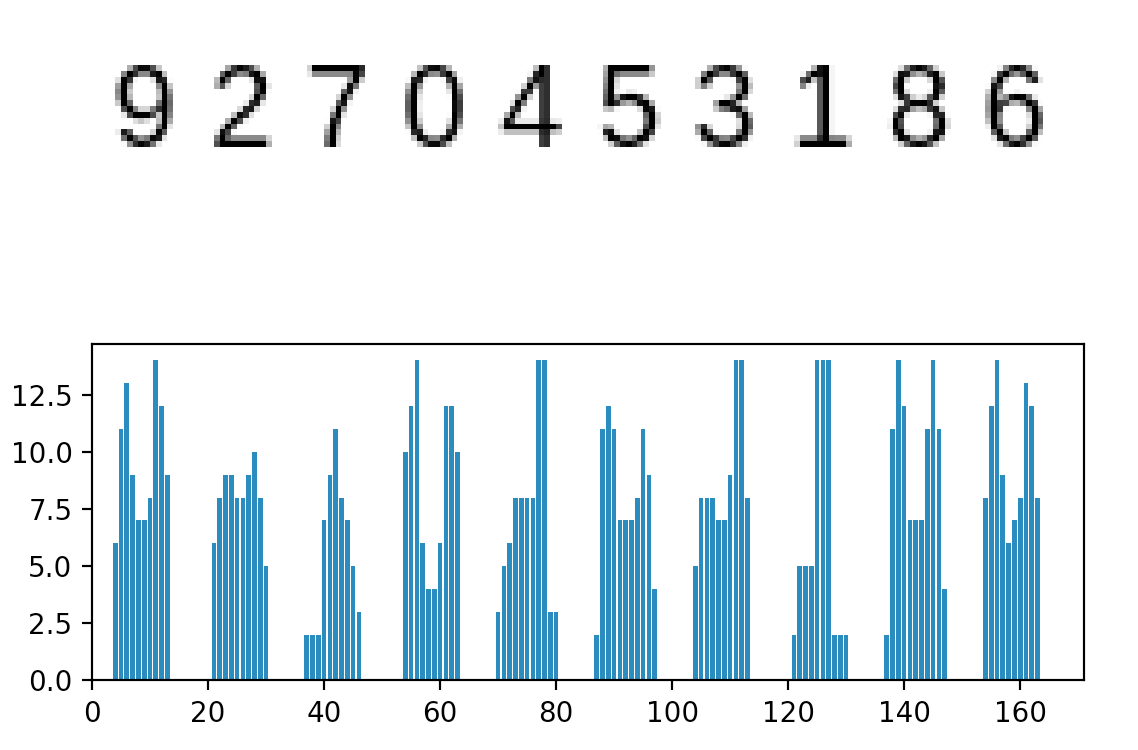
\includegraphics[height=4cm]{res/0-9_segmented_out.png}
    \caption{[0-9] segmented with projection histogram}
    \label{fig:0-9_segmented_out}
  \end{figure}

  \item{Classification - Perceptron neural network - TensorFlow}
    \begin{itemize}
      \item{MNIST dataset - Datasett consisting of several thousand handwritten
      labeled numbers}
      \begin{itemize}
        \item{Numbers ranging from [0-9]}
        \item{Images are 28x28pixels}
      \end{itemize}
      \item{Hyperparameter tuneing}
      \begin{itemize}
        \item{Activation function}
        \item{Number of hidden layers}
        \item{Nodes in hidden layers}
        \item{Cost function}
        \item{Optimazation function}
        \item{Learning rate}
      \end{itemize}
      \item{Theoretic accuracy of the network with 2 hidden layers ~98\%}
      \begin{itemize}
        \item{Measured accuracy ~97\%}

        \begin{figure}[H]
          \centering
          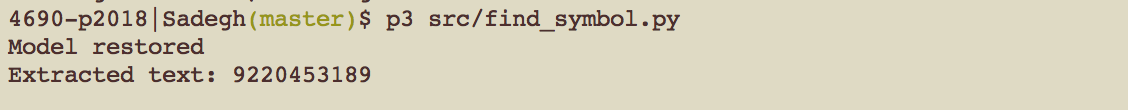
\includegraphics[height=1cm]{res/classification_first_print.png}
          \caption{First output with classification. input see Figure ~\ref{fig:0-9_segmented_out}}
          \label{fig:classification_first_print}
        \end{figure}

      \end{itemize}
    \end{itemize}
\end{itemize}
\end{loggentry}


\newpage
\begin{loggentry}{03.05.18}{Week 3}
\begin{itemize}
  \item{Rotation of text}
  \begin{itemize}
    \item{Hough transform}
    \item{\textit{cv2.minAreaRect()}}
  \end{itemize}
  \item{How to distinguish between upside-down, and verticle vs horisontal text segments}
  \begin{itemize}
    \item{Classifiy in all 4 rotations, and choose the classification with highest avrage confidence}
  \end{itemize}
  \item{Classification - Perceptron neural network - Error}
  \begin{itemize}
    \item{Error rate too high, test-set accuracy 97\%, validation set accuracy $<$ 50\%}
    \item{CNN - TensorFlow Estimator API}
    \begin{itemize}
      \item{Challenging documantation; load/save models}
    \end{itemize}
    \item{Dataset - FNIST - Group contribution}
    \begin{itemize}
      \item{Dataset including several fonts}
      \item{English alphabet, and numbers [0-9]}
    \end{itemize}
  \end{itemize}
\end{itemize}
\end{loggentry}

\newpage
\begin{loggentry}{17.05.18}{Week 4}
\begin{itemize}
  \item{-----}
  \begin{itemize}
    \item{-----}
    \item{-----}
  \end{itemize}
  \item{------}
\end{itemize}
\end{loggentry}

\end{document}
